\subsection{Experiment 2 Results} \label{results-2}
In this section, we first present descriptive statistics of the raw data in the second experiment. Then, we discuss our first analysis on the comparison of relative preference intensity across Likert, QV and Buyback. Lastly, we present our second analysis for comparing the relative preference order across the three groups.

\subsubsection{Descriptive Statistics of the Raw Data}


\begin{table}
    \centering
    \caption{
        Experiment one's sample demographics statistics aligns closely with 2019 US census across all groups and subgroup.
    }
    \Description[Experiment one's sample demographics statistics aligns closely with 2019 US census across all groups and subgroup.]{
        Experiment one's sample demographics statistics aligns closely with 2019 US census across all groups and subgroup.
    }
    \label{table:demo_exp1}
    \begin{tabular}{|c|cccc|c|} 
    \hline
     & \begin{tabular}[c]{@{}c@{}}Likert\\Perc \end{tabular} & \begin{tabular}[c]{@{}c@{}}QV100\\Perc \end{tabular} & \begin{tabular}[c]{@{}c@{}}BuyBack\\Perc \end{tabular} & \begin{tabular}[c]{@{}c@{}}Total\\Perc \end{tabular} & \begin{tabular}[c]{@{}c@{}}Census\\Perc* \end{tabular} \\ 
    \hline
    No High School & 11.32\% & 6.67\% & 7.84\% & 8.72\% & 10.22\% \\
    High School & 28.30\% & 33.33\% & 29.41\% & 30.20\% & 27.73\% \\
    Some College  Associate & 24.53\% & 24.44\% & 27.45\% & 25.50\% & 33.09\% \\
    Bachelor's Degree above & 35.85\% & 35.56\% & 35.29\% & 35.57\% & 33.09\% \\ 
    \hline
    18 - 24 & 7.55\% & 11.11\% & 11.76\% & 10.07\% & 13.65\% \\
    25 - 39 & 33.96\% & 31.11\% & 33.33\% & 32.89\% & 30.74\% \\
    40 - 54 & 26.42\% & 26.67\% & 31.37\% & 28.19\% & 28.32\% \\
    55 - 69 & 32.08\% & 31.11\% & 23.53\% & 28.86\% & 27.29\% \\
    \hline
    \end{tabular}
    \vspace{-10px} %temporary
\end{table}


\subsubsection{Relative Preference Intensity Comparison}

\begin{figure}[htpb]
  \centering
  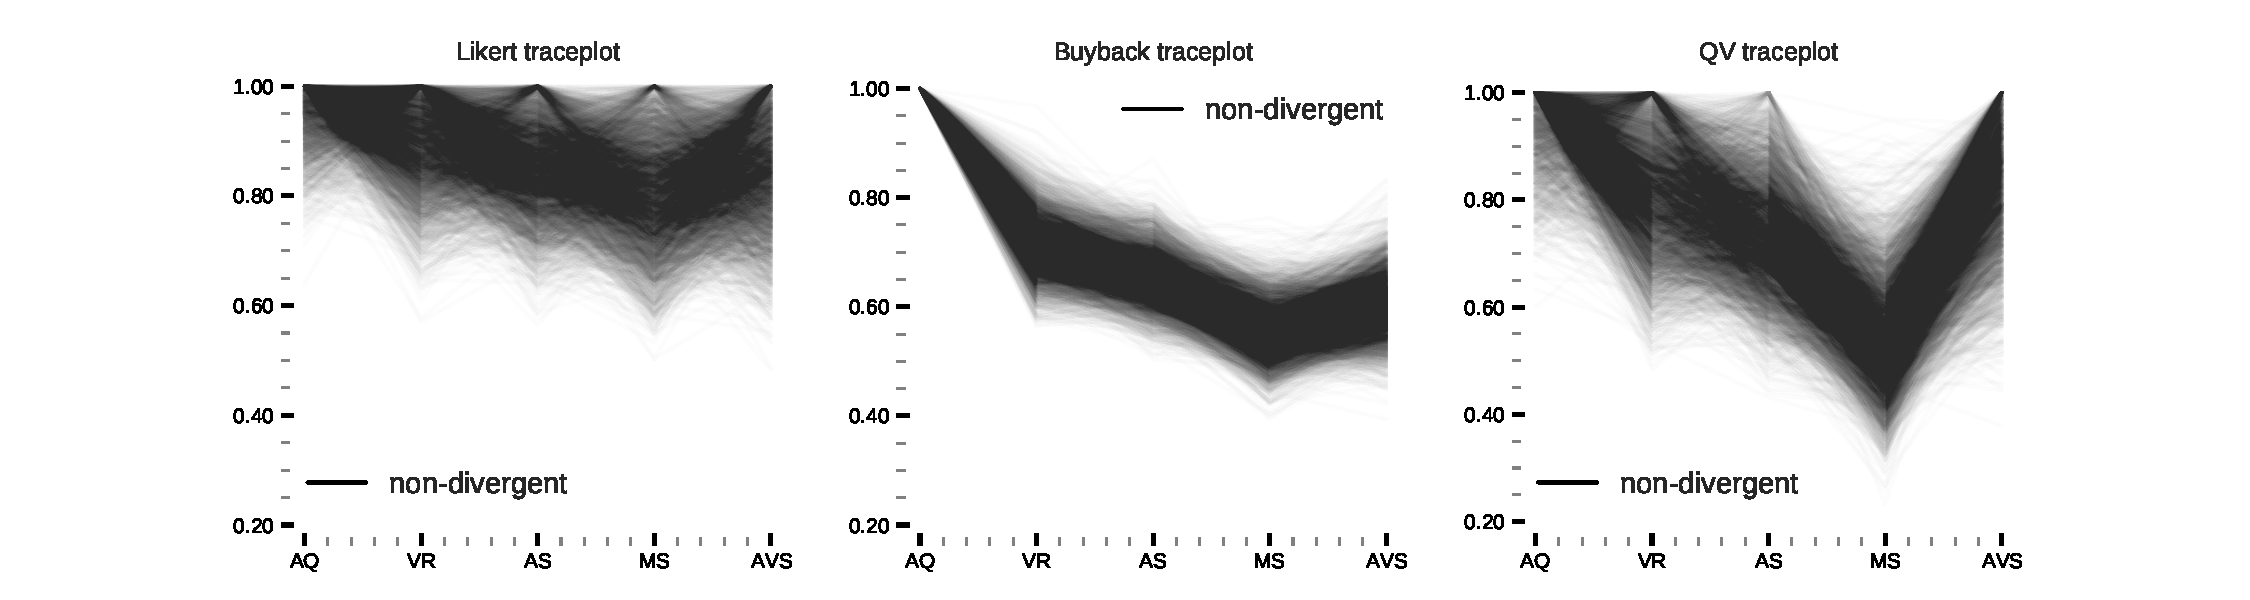
\includegraphics[trim= 1.5in 0in 1.5in 0in, clip, width=\textwidth, keepaspectratio=true]{"content/image/exp2_2_means_traceplot.pdf"}
  \caption{
    The figure shows comparison of the sampling traces of normalized means from Likert, QV and Buyback's Bayesian models. The models model on Likert's votes between [$-2$, $2$], QV's signed-credits between [$-100$, $100$], and Buyback proportions between [$0$, $1$] respectively. Means from the three Bayesian models are normalized to [$-1$, $1$] by the value of their maximum dimension in every trace respectively for this graph. The mapping of the labels on X-axis are: AQ -- Audio Quality, VR -- Video Resolution, AS -- Audio Stability, MS -- Motion Smoothness, AVS -- Audio-video Sync. QV's traces resemble those of Buyback more than Likert. Most of Likert's traces are above 0.8, showing consistent high intensities across aspects. Both QV and Buyback show a greater variation in the relative intensities and have a significant amount of traces dipping down to the range of 0.4 to 0.6 for the least popular aspect.
  }
  \Description[Means traceplots for exp2]{Means traceplots for exp2}
  \label{fig:means_exp2}
\end{figure}

\subsubsection{Relative Preference Order Comparison}